%%%%% Physik Kompendium Nr.2 %%%%%
%% 02 -- Generator %%


\subsection{Funktionsprinzip}

Eine Spule, oder der Anschaulichkeit wegen, eine Leiterschleife, befindet sich in einem magnetischen Feld (Siehe Abbildung).\footnote{LeiFi Physik, Genommen von: \url{http://www.leifiphysik.de/sites/default/files/medien/generator02_elmagnetindukt_ver.gif}}

\begin{figure}[h!]
	\centering
	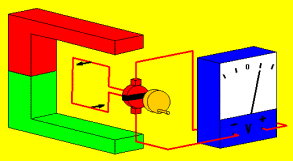
\includegraphics[width=0.5\textwidth]{Pictures/GeneratorSchema}
	\caption{Schema eines Wechselstromgenerators mit Kommutator} 
\end{figure}



Die Leiterschleife dreht sich, und der zur Aufnahmezeit sich oben befindende Teil der Schleife bewegt sich senkrecht zu den Feldlinien des Magnetfeldes und somit wirkt auf die Teilchen die Lorentzkraft, gemäß Linker-Hand-Regel. Im Beispiel ist der Plus-Pol am oberen Ende und der Minus-Pol am unteren Ende.

Wenn sich die Schleife nun um 90\degree{} dreht, bewegen sich beide Pole parallel zu den Feldlinien; es liegt keine Spannung an. Der Sinusförmige Spannungsgraf resultiert aus der Bewegung dazwischen.

Nach weiteren 90\degree{} ist das ursprünglich obige Stück Schleife unten und nun der Minus-Pol. Das ist der Grund für die negativen Passagen der Spannungskurve. \\
\vspace{11pt}
Ein Kommutator, wie in der Abbildung, kehrt die Polarität der Leiterschleifenteile bei jeder halben Umdrehung um, sodass es nie eine negative Spannung gibt. Die Spannungskurve ist dann der Betrag: $|\sin x|$ Dieses Bauteil wird nicht weiter betrachtet.



\subsection{Induktionsspannung bestimmen}

Um die maximale Spannung (Amplitude), zu bestimmen, muss die Feldstärke des Magnetfeldes, die Windungszahl, Fläche und Induktivität der Spule sowie die Drehfrequenz bekannt sein. Die Gleichung ist analog zur generellen Induktionsspannung $U_{ind} = -N \frac{d(B \cdot A)}{dt}$:

\begin{equation}	\label{eq:hatU}
	\hat{U} = NBA \ \omega
\end{equation}

Daraus folgt für einen beliebigen Zeitpunkt:

\begin{align}		\label{eq:hatUbeliebig}
\begin{split}
	U(t) &= \hat{U} \cdot sin(\omega \cdot t) \\
	U(t) &= NBA \ \omega \cdot sin(\omega \cdot t)
\end{split}
\end{align}



